\documentclass[a4paper]{article}
\usepackage{fullpage}
\usepackage{amssymb}
\usepackage{amsmath}
\usepackage{graphicx}


\title{Coursework: Divide and Conquer -- Report}


\begin{document}
\maketitle

\section*{Latex Examples}

\begin{figure}[h]

\includegraphics[width=0.48\linewidth]{example_plot1.png}
\includegraphics[width=0.48\linewidth]{example_plot2.png}

\caption{Example for embedding plots in Latex.}
\label{fig:examples}
\end{figure}


\section{Recurrences}

\subsection{Substitution Method}

Recursion trees allow you to analyse recurrences to obtain a guess for the substitution method. A closely related method is to expand out the recurrence a few times, until a pattern emerges. We call this the expansion method. An example of how to use the expansion method is given below.\\
\newline
Use the expansion method to guess an upper bound and the substitution method to verify your guess:

\begin{itemize}

\item Example: $T(n) = 2T(n/2) + n$

Introduce constants $c$ and expand the recurrence: \\
\begin{align*}
T(n) & \leq 2T(n/2) + cn \\
~ & \leq 2[2T(n/4) + cn/2] + cn = 4T(n/4)+2cn \\
~ & \leq 4[2T(n/8) + cn/4] + 2cn = 8T(n/8)+3cn \\
~ & \leq 8[2T(n/16) + cn/8] + 3cn = 16T(n/16)+4cn \\
~ & \vdots
\end{align*}

A pattern is emerging. The general term is $T(n) \leq 2^k T(n/2^k) + kcn$. Plugging in $k=\lg n$ (the height of the recursion tree), we get $T(n) \leq nT(1) + cn \lg n = O(n \lg n)$.\\
\newline
Now we verify $O(n \lg n)$ using the substitution method:\\
\newline
Prove that
\begin{align*}
T(n) \leq c(n \lg n)
\end{align*}
Assume that
\begin{align*}
T(\frac{n}{2}) \leq c(\frac{n}{2} \lg \frac{n}{2})
\end{align*}
By substitution
\begin{align*}
T(n) & \leq 2(c(\frac{n}{2} \lg \frac{n}{2})) +  n \\
~ & = cn \lg \frac{n}{2} + n \\
~ & = cn \lg n - cn \lg 2 + n \\
~ & \leq cn \lg n \quad \text{holds for} \, c \geq 1 \\
\end{align*}

\item $T(n) = 3T(n/2) + n$ 

Insert your solution here

\item $T(n) = T(n/2) + n^2$

Insert your solution here

\item $T(n) = 4T(n/2 + 2) + n$

Insert your solution here

\item $T(n) = 2T(n-1) + 1$

Insert your solution here

\item $T(n) = T(n-1) + T(n/2) + n$

Insert your solution here

\end{itemize}

\subsection{Master Method}

Use the master method to give tight asymptotic $\Theta$ bounds:

\begin{itemize}

\item Example: $T(n) = 2T(n/2) + n$

Cost at leaves: $\Theta(n^{\log_b a}): n^{\log_2 2}=n=\Theta(n)$ \\
Cost per depth: $f(n)=n$ \\
Case 2: $f(n) = \Theta(n^{\log_b a})$: $f(n) = \Theta(n)$ \\
Solution: $\Theta(n^{\log_b a} \lg n) = \Theta(n \lg n)$

\item $T(n) = 2T(n/4) + 1$

Insert your solution here

\item $T(n) = 2T(n/4) + n$

Insert your solution here

\item $T(n) = 2T(n/2 + 17) + n$

Insert your solution here

\item $T(n) = 4T(n/2) + 2^n$

Insert your solution here

\item $T(n) = T(3n/4) + \sqrt{n}$

Insert your solution here

\end{itemize}

\section{Sorting}

\subsection{Plots}

Insert your plots here

\subsection{Discussion}

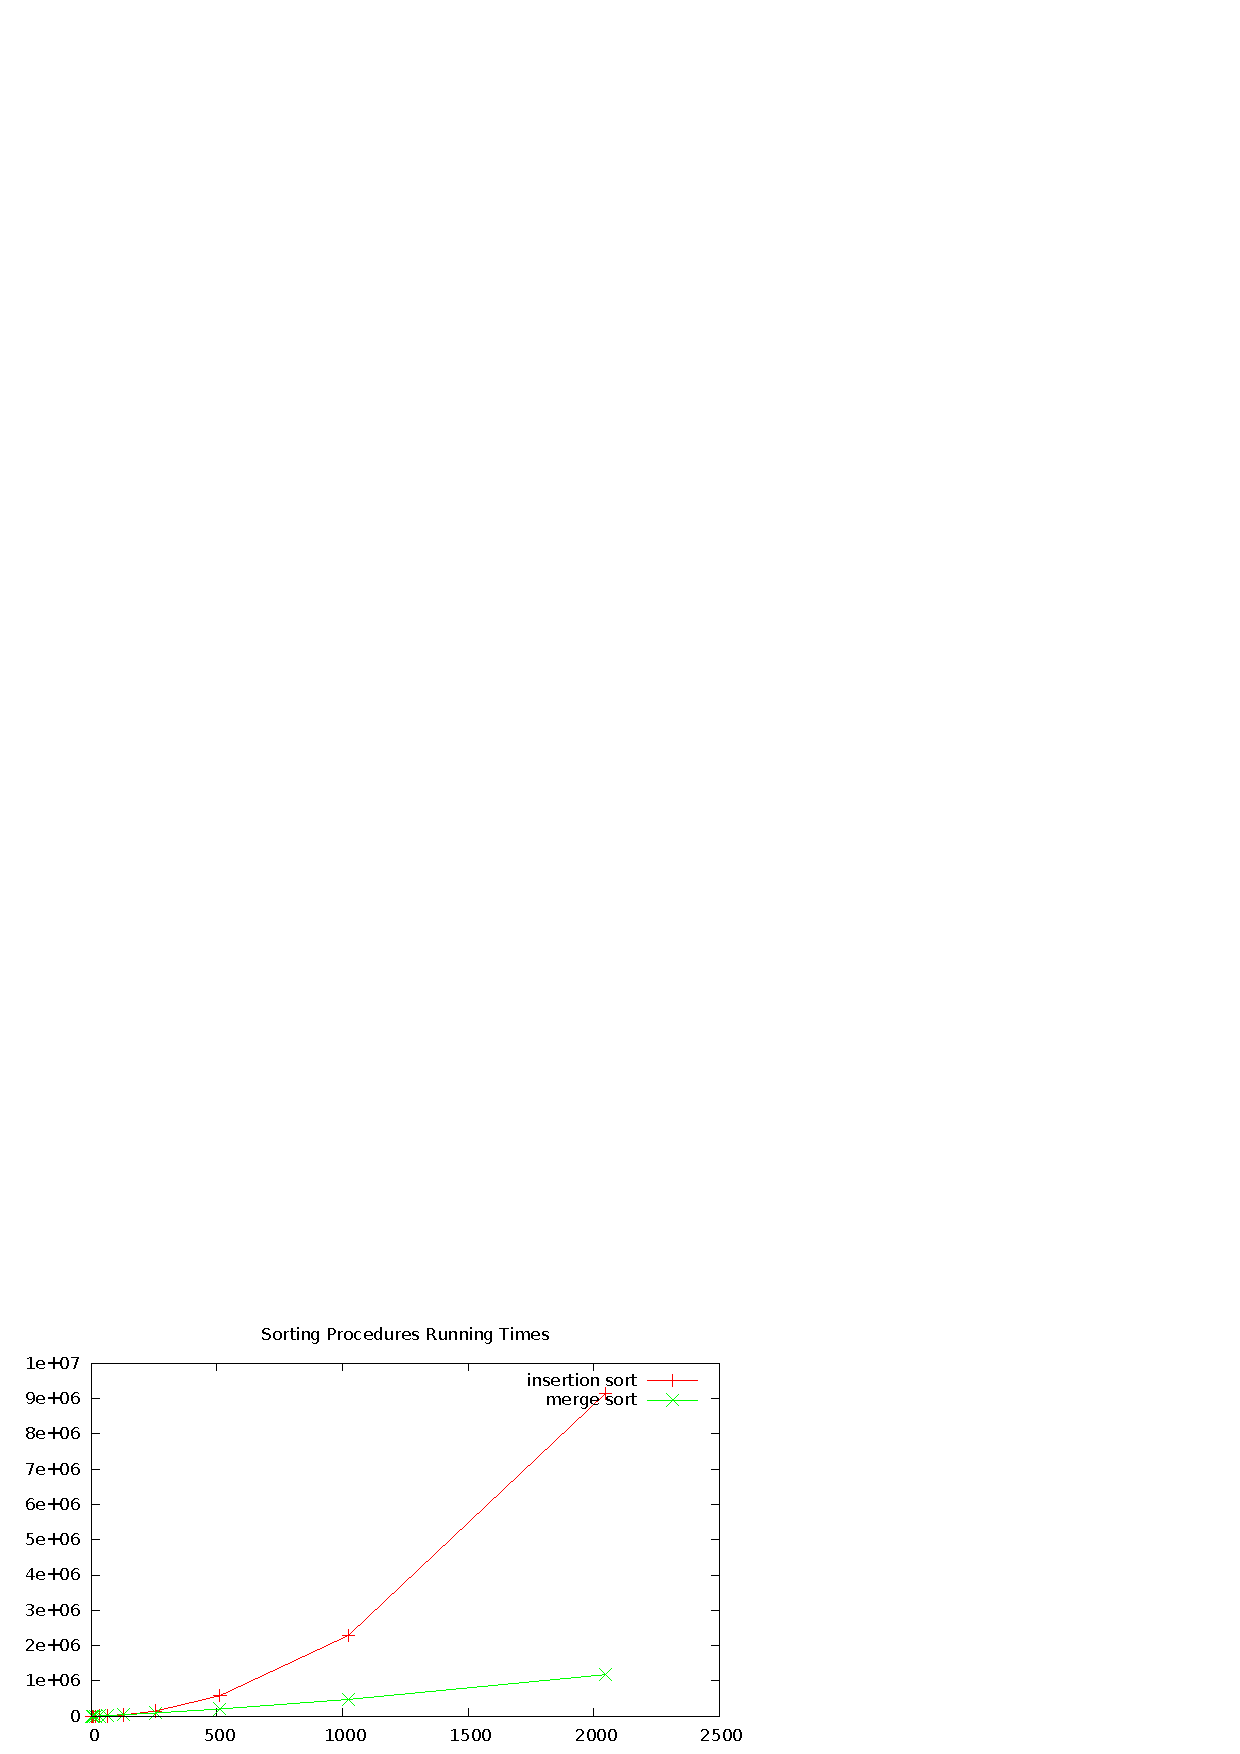
\includegraphics[width=0.48\linewidth]{sort_insert_vs_merge.png}

Insertion sort is faster than merge sort on small arrays up to size 8.
That is because at every run of MergeSort::sortpart(), the subarray is copied, which takes time that is linear in the length of the subarray. Since the recursion tree has depth $\log_2 n$, each entry is copied $\log_2 n$ times so this array copying altogether takes $\Theta(n^{\log_2 n})$ time. On the other hand, insertion sort does not do any array copying (but moving an entry to its correct position takes \mathcal{O}(n) time).\\

\includegraphics[width=0.48\linewidth]{sort_all_hybrid-bad.png}

One would think that hybrid sort would therefore be optimal by running pure insertion sort when array size less than 8, and pure merge sort otherwise. Results are above. The code for this version of hybrid sort can be found in BadHybridSorts.cpp as sorta().\\

\includegraphics[width=0.48\linewidth]{sort_all_hybrid-threshold8.png}

But we can do better: since merge sort breaks down array into smaller arrays, and for sufficiently small arrays, insertion sort is better, maybe insertion sort should always be used 'towards the end' of hybrid sort to achieve better results. Results are above. The code for this version of hybrid sort can be found in BadHybridSorts.cpp as sortb().\\

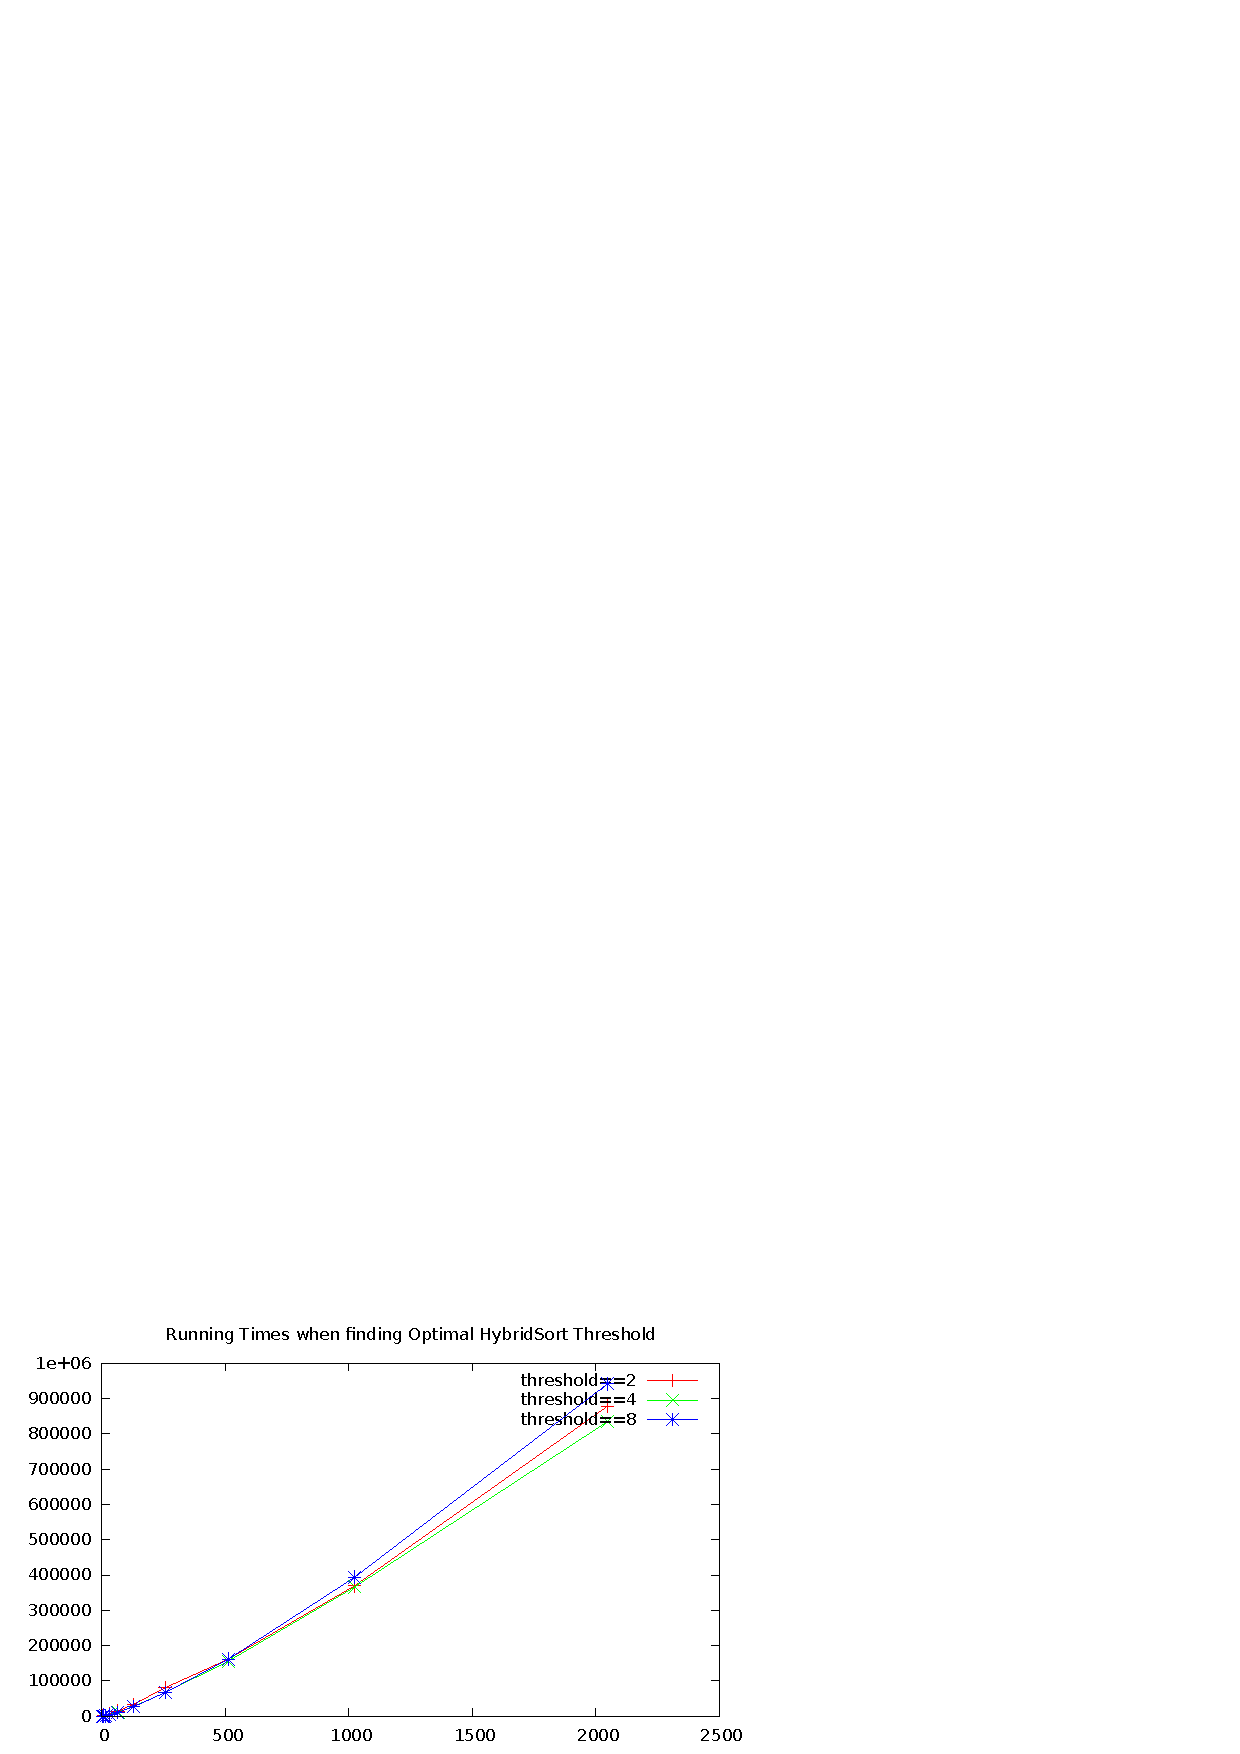
\includegraphics[width=0.48\linewidth]{sort_hybrid_thresholds.png}

We can do better: it's not because insertion is better up to size 8 that it should be used as soon as size is 8. Maybe merge should break array down to, say, subarrays of size 4, and insertion should act on that. There would be more breaking down, but maybe this is more than compensated by just how much faster insertion is per average entry on arrays of size 4 vs arrays of size 8. We tried various different threshold array sizes, and the best was found to be for size 2. Results are above. The code for these versions of hybrid sort can be found in HybridSorts.cpp as sortb(). The final plot comparing insertion sort, merge sort, and optimal hybrid sort is below. \\

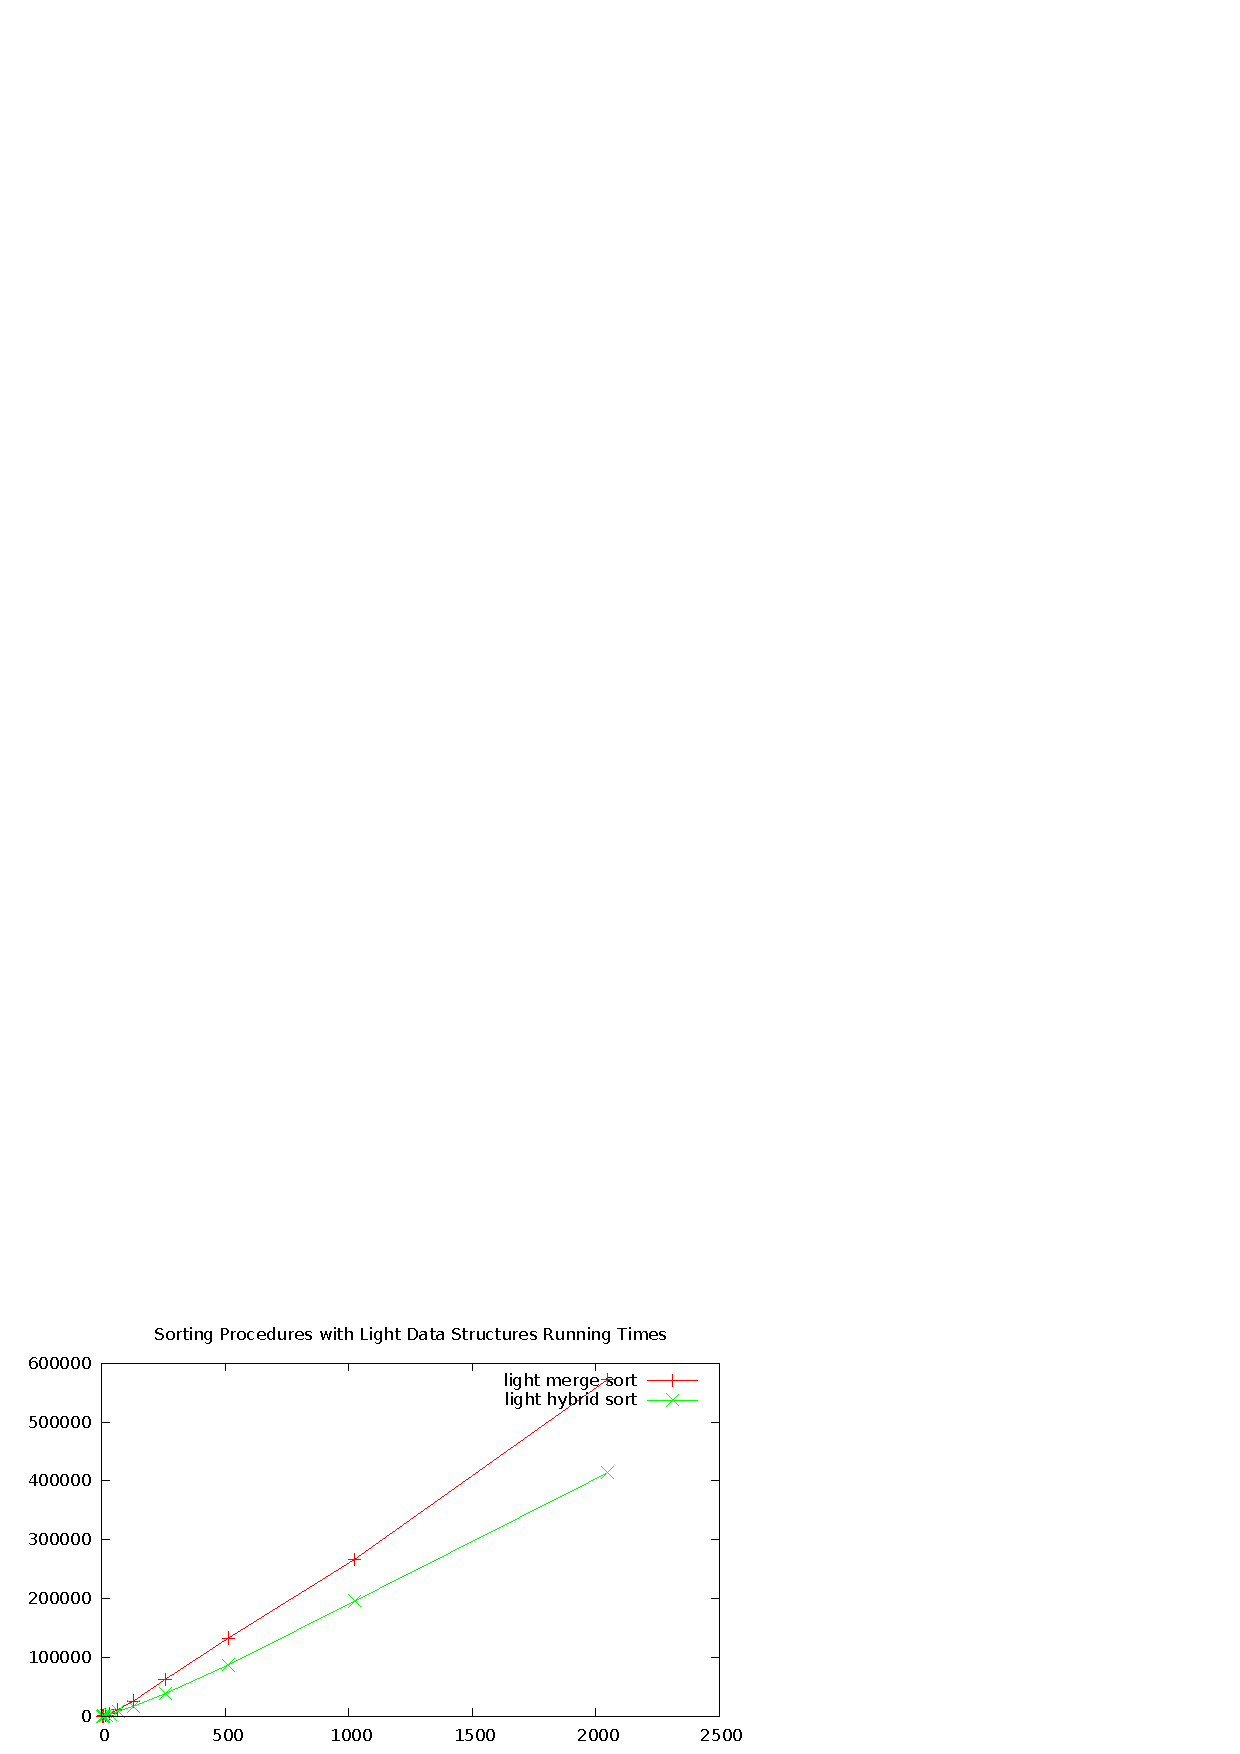
\includegraphics[width=0.48\linewidth]{sort_final.png}

As an extension, merge sort can be improved by using a lighter data structure when copying the entries: in this case, a static array is used instead of a vector. (We found that using a static array was faster than using a dynamic array. Maybe this is because OS operations on the heap are slower than on the stack?) In this case, merge sort beats insertion sort on any array size, so it no longer makes sense to combine the two in hybrid sort, i.e. hybrid sort is optimal when it always runs pure merge sort. Results are below. The code for these versions of merge sort and hybrid sort can be found in LightSorts.cpp as lightmergesort() and lighthybridsort().\\

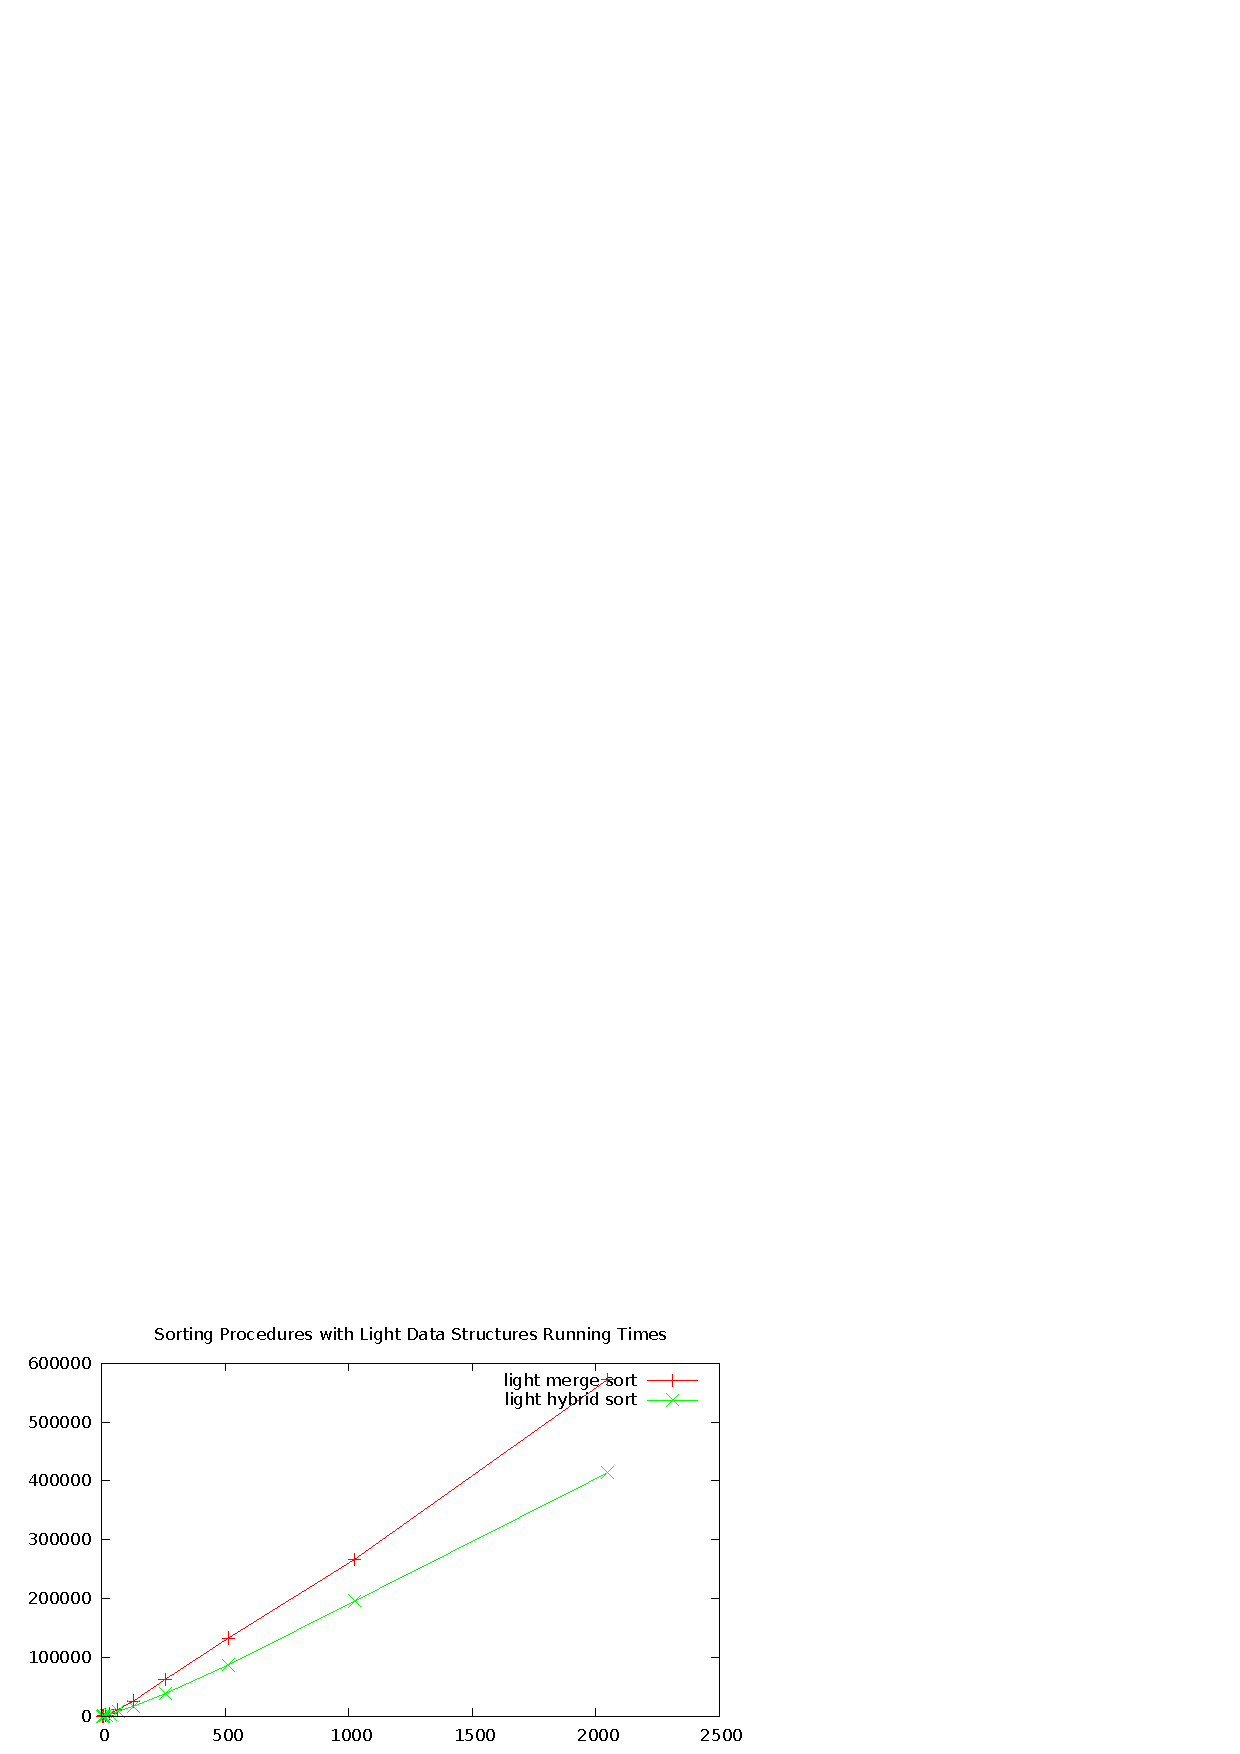
\includegraphics[width=0.48\linewidth]{sort_lights.png}


\section{Integer Multiplication}

\subsection{Plots}

\noindent Insert your plots here

\subsection{Discussion}

\noindent Insert your discussion here

\subsection{Recurrences}

\subsubsection{Recursive Multiplication}

\noindent Insert your solution here

\subsubsection{Karatsuba Multiplication}

\noindent Insert your solution here

\end{document}
